\documentclass[11pt]{article}

\usepackage[margin=1in]{geometry}
\usepackage{amsmath,amssymb,amsthm}
\usepackage{graphicx}
\usepackage{booktabs}
\usepackage{xcolor}
\usepackage[numbers,sort&compress]{natbib}
\usepackage[colorlinks=true,linkcolor=black,citecolor=blue,urlcolor=blue]{hyperref}

\graphicspath{{figures/}}
\setlength{\emergencystretch}{2em}
\newcommand{\Sig}{\Sigma}
\newcommand{\Sighat}{\widehat{\Sigma}}
\newcommand{\muhat}{\widehat{\mu}}
\newcommand{\TN}{T/N}

\title{\bfseries When Does Hierarchical Risk Parity Beat Markowitz?\\
A Controlled Comparison Under Known Covariance}

\author{Eugen Soloviov\thanks{Independent Researcher. ORCID:
\href{https://orcid.org/0009-0006-3148-111X}{0009-0006-3148-111X}.
Correspondence: \href{mailto:suenot@gmail.com}{suenot@gmail.com}.
Code to reproduce every number and figure:
\url{https://github.com/suenot/hrp-validation}.}}

\date{}

\begin{document}
\maketitle

\begin{abstract}
Hierarchical Risk Parity (HRP) replaces covariance-matrix inversion with
hierarchical clustering and recursive inverse-variance allocation, and is
widely promoted as the practical cure for the instability of Markowitz
optimization. We give this claim a controlled test in which the \emph{true}
covariance matrix is known by construction, so the realized risk of any weight
vector is computable exactly as $w^{\top}\Sig w$ and the unconstrained
minimum-variance oracle is an exact floor. Across $4{,}800$ experiments
($4{,}000$ Gaussian, $800$ multivariate Student-$t$) spanning four
true-correlation families---one-factor, nested hierarchical, unstructured
(normalized Wishart), and equicorrelation---with $N\in\{10,\dots,100\}$ assets
and estimation windows of $\TN\in[0.5,10]$, the verdict splits cleanly.
(i)~HRP's \emph{insurance value against naive Markowitz is real}: at $T=N$,
where the sample covariance is singular, sample minimum variance realizes a
median $16.8\times$ the oracle risk (above $100\times$ in $9\%$ of cases),
while HRP realizes $2.3\times$, beats sample minimum variance in $87\%$ of
data-starved experiments ($\TN\le1$; every single one in the unstructured
family at $\TN=0.5$), and never suffers an inversion catastrophe.
(ii)~\emph{Its advantage over shrinkage is mostly not}: Ledoit--Wolf
minimum variance---equally inversion-proof, one line of
scikit-learn---realizes $1.8\times$ at $T=N$ and beats HRP at every $\TN$ in
the factor, hierarchical, and equicorrelation families; HRP's win rate
against it is $0.34$ at $\TN\le1$ and falls to $0.05$ at $\TN\ge5$, with HRP
ahead only under unstructured correlation at small $T$ (win rate
${\approx}0.55$). The $1.8$-versus-$2.3$ comparison pits shorts-allowed LW
against long-only HRP; on the like-for-like long-only comparison at $T=N$
the pooled medians are a near-tie (clipped LW $2.32\times$ vs.\ HRP
$2.29\times$), though LW remains ahead in paired comparisons.
(iii)~HRP is \emph{not a consistent minimum-variance
estimator}: by $\TN=10$ sample and shrunk minimum variance converge to
${\approx}1.10\times$ the oracle while HRP plateaus at $1.40$--$3.20\times$
depending on family. (iv)~Much of HRP's behavior is the inverse-variance
portfolio inside it: in the data-starved band its win rate against diagonal
inverse variance exceeds $0.5$ only when clusters genuinely differ in
tightness (rising $0.35\to0.56$ across dispersion terciles of our
hierarchical worlds), in the data-rich band it edges IV more broadly (win
rates $0.46$--$0.63$ at $\TN\ge5$), and the much-debated linkage choice is
immaterial (the three linkage medians agree to within $0.02$--$0.06$). (v)~Estimated \emph{means}, not estimated
covariances, remain the real catastrophe: tangency portfolios built from
estimated means capture a median $10\%$ of the oracle Sharpe ratio at
$\TN\le1$ and are negative $28\%$ of the time. The Student-$t$ batch leaves
every qualitative ranking unchanged. Practical reading: HRP is real
insurance against inverting a noisy covariance matrix when the correlation
structure is unknown and data are scarce---but if you can shrink, shrinking
is better almost everywhere.
\end{abstract}

\section{Introduction}

Markowitz mean--variance optimization \citep{markowitz1952portfolio} is
provably optimal with known inputs and notoriously fragile with estimated
ones: the optimizer amplifies exactly the estimation errors that matter most
\citep{michaud1989markowitz,best1991sensitivity,chopra1993effect}. The most
influential recent response in practitioner circles is Hierarchical Risk
Parity \citep[HRP;][]{lopezdeprado2016building}, which never inverts a
matrix: it clusters assets by correlation distance, reorders the covariance
into quasi-diagonal form, and allocates top-down by recursive
inverse-variance bisection. HRP is now a default in several open-source
portfolio libraries and is routinely recommended as the robust replacement
for Markowitz.\footnote{Including in the author's own earlier practitioner
writing, where the exact pipeline tested here---single-linkage clustering on
correlation distance, quasi-diagonalization, recursive inverse-variance
bisection---was recommended over Markowitz inversion for allocating capital
across market-making strategies. This paper is therefore a controlled
self-audit of advice the author has himself circulated, not an attack on a
third party.}

The evidence behind the recommendation is thinner than its adoption. The
original paper demonstrates HRP on one numerical example and one Monte Carlo
design, against unshrunk benchmarks; most follow-ups are empirical backtests
in which the true covariance is unknown, so no one can say how far any
allocator sits from the attainable optimum, or how much of its loss is
estimation error versus specification error. Meanwhile the estimation-error
literature has its own well-validated remedy---shrinkage
\citep{ledoit2003improved,ledoit2004well,ledoit2004honey}---which is almost
never the benchmark HRP is compared against.

This paper supplies the missing controlled comparison. We generate the true
covariance $\Sig$ from four structural families chosen to span the cases
where HRP's clustering prior is right (nested hierarchical blocks), partially
right (one common factor), and wrong (unstructured dense correlation;
equicorrelation), hand every allocator the same finite sample of $T$
observations, and score the resulting weights \emph{on the truth}: realized
risk $w^{\top}\Sig w$ against the exact unconstrained minimum-variance
oracle. There is no backtest noise and no data snooping; the only randomness
is the sampling error every estimator faces. We sweep the ratio $\TN$ from
$0.5$ (deeply singular) to $10$ (data-rich), because the
break-even results of \citet{demiguel2009optimal} identify exactly this
ratio as the axis on which optimization beats naive rules.

Our findings are deliberately mixed, and more useful for it. HRP's headline
story---``Markowitz explodes, HRP does not''---is confirmed, and
quantified: at $T=N$ the sample minimum-variance portfolio realizes a median
$16.8\times$ the oracle risk, HRP $2.3\times$. But the comparison that
practitioner writing rarely runs---HRP against Ledoit--Wolf shrinkage, which
is equally inversion-proof and one line of scikit-learn---reverses the
story almost everywhere: shrinkage wins at every $\TN$ in three of our four
families, and HRP's edge survives only where there is no structure for its
dendrogram to find and very little data to estimate with. Linkage choice,
the subject of a sizable applied debate, moves the median result by
$0.02$--$0.06$ depending on family; the dispersion of cluster tightness,
which nobody debates, moves HRP's data-starved win rate against its own
inverse-variance core from $0.35$ to $0.56$.
And the classical disaster remains where \citet{demiguel2009optimal} located
it: portfolios that estimate \emph{means} capture a median $10\%$ of the
attainable Sharpe ratio in the data-starved regime and are negative $28\%$
of the time.

\paragraph{Contributions.}
\begin{enumerate}\itemsep2pt
\item A reproducible known-covariance testbed for portfolio allocators: four
true-correlation families with every generator parameter drawn from one
disclosed sampling table and recorded per experiment, Gaussian and
multivariate Student-$t$ returns, and exact evaluation of realized risk
$w^{\top}\Sig w$ against the exact minimum-variance oracle
(Sections~\ref{sec:allocators}--\ref{sec:setup}).
\item A quantification of HRP's insurance value against naive Markowitz in
the data-starved regime, and of its failure to converge in the data-rich
regime: HRP's realized-risk plateau at $1.40$--$3.20\times$ the oracle
isolates its specification gap, the loss it would retain even with the true
covariance (Sections~\ref{sec:starved}--\ref{sec:rich}).
\item The comparison that matters and is rarely run: HRP versus Ledoit--Wolf
shrinkage, stratified by structure family and $\TN$, with win rates and
paired log-ratios. Shrinkage wins almost everywhere; we delineate the
exception (unstructured correlation, $\TN\le1$) and show that even there
plain inverse variance is better still (Section~\ref{sec:shrinkage}).
\item Evidence on \emph{which} of HRP's ingredients matter: cluster-tightness
dispersion does (data-starved win rate vs.\ inverse variance $0.35\to0.56$
across terciles), linkage does not (the three linkage medians agree to
within $0.02$--$0.06$, and the distance-matrix convention behind the linkage
moves them by at most $0.02$), and HRP's turnover and concentration profile
is closer to inverse variance than to any optimizer
(Sections~\ref{sec:ivp}--\ref{sec:linkage}).
\item A replication, inside the same harness, of the classical result that
estimated means are the dominant failure mode: noisy-$\mu$ tangency
directions capture a median $10\%$ of the oracle Sharpe at $\TN\le1$,
negative in $28\%$ of experiments---below every $\mu$-free rule in the same
regime, from sample minimum variance ($18\%$ pooled) to the diffuse rules of
Table~\ref{tab:sharpe} ($26$--$70\%$) (Section~\ref{sec:mu}).
\end{enumerate}

\section{Related work}
\label{sec:related}

\paragraph{Estimation error in mean--variance optimization.}
Mean--variance portfolio selection \citep{markowitz1952portfolio} is optimal
only when its inputs are known; in practice they must be estimated, and the
optimizer interacts badly with estimation noise. \citet{jobson1980estimation}
showed in early Monte Carlo experiments that sample-based efficient
portfolios can be dramatically inferior to the population-optimal ones, and
\citet{jobson1981putting} argued that naive alternatives are often preferable
in realistic sample sizes. \citet{michaud1989markowitz} popularized the
diagnosis of mean--variance optimizers as ``estimation-error maximizers''
that load on the most extreme---and most mis-estimated---inputs. Subsequent
work quantified the mechanism: optimal weights are extremely sensitive to
small perturbations of expected returns \citep{best1991sensitivity}, errors
in means dominate but covariance errors matter increasingly at high risk
tolerance \citep{chopra1993effect}, and even with optimal Bayesian use of
sample information, parameter uncertainty erodes most of the theoretical
gains from optimization \citep{kan2007optimal}. The starkest statement of the
problem is due to \citet{demiguel2009optimal}: across fourteen optimizing
models and seven empirical datasets, none consistently outperforms the
equally weighted $1/N$ portfolio out of sample, because the estimation window
needed for sample-based mean--variance to win is far longer than anything
available in practice. Their analysis ties the break-even point explicitly to
the ratio of sample size to universe size---the same $\TN$ axis we stratify
on.

\paragraph{Covariance-focused remedies.}
One response is to abandon expected-return estimation and target the
minimum-variance portfolio, which depends only on the covariance matrix and
has performed well empirically \citep{clarke2006minimum,clarke2011minimum}.
But the covariance matrix itself is noisy when $N$ is large relative to $T$.
Random matrix theory shows that the bulk of sample correlation eigenvalues
from financial data is indistinguishable from noise
\citep{laloux1999noise,plerou1999universal}, motivating a large literature on
eigenvalue cleaning \citep{bun2017cleaning}. Shrinkage estimators address the
same ill-conditioning by pulling the sample covariance toward a structured
target---a single-factor model \citep{ledoit2003improved}, a scaled identity
with asymptotic optimality guarantees \citep{ledoit2004well}, or the
constant-correlation target of the widely used ``Honey, I shrunk'' estimator
\citep{ledoit2004honey}. \citet{jagannathan2003risk} showed that no-short-sale
constraints act as an implicit shrinkage of extreme covariances, which
explains why constrained sample-based minimum-variance portfolios perform
respectably. This literature establishes that \emph{how} the covariance is
estimated matters; it says less about how the optimizer's sensitivity to the
remaining error depends on the structure of the true covariance.

\paragraph{Hierarchical portfolio construction.}
A parallel line, rooted in the observation that financial correlation
matrices carry a hierarchical organization \citep{mantegna1999hierarchical},
sidesteps matrix inversion altogether. Hierarchical Risk Parity
\citep{lopezdeprado2016building} clusters assets with single-linkage
agglomerative clustering on a correlation distance, quasi-diagonalizes the
covariance, and allocates by recursive inverse-variance bisection.
\citet{raffinot2017hierarchical} proposed hierarchical clustering-based
allocation with alternative linkages and equal weighting across clusters,
later extended to hierarchical equal risk contribution in a working paper
\citep{raffinot2018herc}. Further extensions incorporate
tail-dependence-based distances in multi-asset multi-factor settings
\citep{lohre2020hierarchical}, constraints and a continuum between
cluster-level and asset-level allocation \citep[a working
paper]{pfitzinger2019constrained}, and Monte-Carlo-based modifications for
managed futures \citep{molyboga2020modified}. \citet{jaeger2021interpretable}
use explainable-machine-learning tools to attribute when and why HRP-type
strategies beat equal weight in block-bootstrapped multi-asset data. Most
recently, \citet{cotton2024schur} showed that HRP and minimum variance are
endpoints of a single family of Schur-complement allocations, sharpening the
question of where on that spectrum one should sit---a question whose answer
must depend on estimation error.

\paragraph{The gap.}
The original evidence for HRP consists of one numerical example and one Monte
Carlo experiment with a particular block-diagonal-plus-shocks data-generating
process, evaluated against unshrunk inverse-variance benchmarks
\citep{lopezdeprado2016building}. Follow-up studies are predominantly
empirical backtests
\citep{raffinot2017hierarchical,lohre2020hierarchical,jaeger2021interpretable},
where the true covariance is unknown, so realized out-of-sample variance
confounds estimation error with model misspecification and nonstationarity,
and no oracle is available to measure either. Meanwhile, the $1/N$ literature
\citep{demiguel2009optimal} and the shrinkage literature
\citep{ledoit2004honey,ledoit2004well} each demonstrate their preferred
remedy on their own testbeds, with no common ground truth. What is missing is
a controlled comparison in which the true covariance is known by construction
and varied systematically across structural families---strict factor models,
genuinely hierarchical block structures, unstructured dense matrices, and
equicorrelation---while the sample length $T$ and universe size $N$ are swept
over the $\TN$ ratios that drive the DeMiguel-style break-even results.
Against the known-covariance oracle, the excess realized risk of each
portfolio rule decomposes cleanly into a specification term (what the rule
would lose even with perfect inputs, relevant for HRP and $1/N$, which are
not oracle-optimal) and an estimation term (what it loses to sampling noise).
To our knowledge no published study reports this decomposition for HRP
against sample and Ledoit--Wolf-shrunk minimum variance, inverse variance,
and $1/N$ across structures and $\TN$ regimes, nor does any systematically
examine HRP's sensitivity to the linkage rule, despite the well-documented
chaining behavior of single linkage \citep{murtagh2012algorithms} and
Raffinot's evidence that linkage choice materially changes hierarchical
allocations \citep{raffinot2017hierarchical}. This paper fills that gap.

\section{Allocators}
\label{sec:allocators}

Every allocator maps an estimation window
$R\in\mathbb{R}^{T\times N}$ (or the sample covariance built from it) to
full-investment weights, $\sum_i w_i = 1$; all are scored on the true
$\Sig$. The risk-only track contains ten methods that never see a mean
estimate.

\paragraph{Equal weight (EW).} $w_i = 1/N$, the
\citet{demiguel2009optimal} benchmark.

\paragraph{Inverse variance (IV).} $w_i \propto 1/\Sighat_{ii}$, the
diagonal-only allocator. It is the degenerate HRP that ignores all
correlation information, and therefore the cleanest control for how much
HRP's clustering machinery adds.

\paragraph{Sample minimum variance (MV).} The closed-form unconstrained
minimizer of $w^{\top}\Sighat w$ subject to $\mathbf{1}^{\top}w=1$,
\begin{equation}
w_{\mathrm{MV}} \;=\; \frac{\Sighat^{+}\mathbf{1}}
{\mathbf{1}^{\top}\Sighat^{+}\mathbf{1}},
\label{eq:minvar}
\end{equation}
shorts allowed, with $\Sighat$ the sample covariance
(\textsc{ddof}=1). When $T\le N$ the sample covariance is singular; we use
the Moore--Penrose pseudoinverse (the minimum-norm solution) and flag the
record as rank-deficient rather than failing, since this is exactly the
regime in which the HRP debate lives. The pseudoinverse truncates at NumPy's
default relative cutoff ($\texttt{rcond}=10^{-15}$); the $16.8\times$
headline of Section~\ref{sec:starved} is insensitive to this choice:
replaying every $\TN=1$ experiment with cutoffs
$10^{-15}/10^{-10}/10^{-6}/10^{-3}$ gives pooled medians
$16.82/16.82/15.61/3.98$, so only an absurdly aggressive cutoff---itself a
crude regularizer---changes the picture.

\paragraph{Long-only clip (MV-LO).} Negative weights clipped to zero, then
renormalized. This is deliberately the crude practitioner heuristic, not the
long-only quadratic program: it is what naive implementations do, and the
implicit-shrinkage result of \citet{jagannathan2003risk} suggests even this
crude projection should help.

\paragraph{Ledoit--Wolf minimum variance (LW, LW-LO).} Equation
\eqref{eq:minvar} applied to the shrinkage estimator of
\citet{ledoit2004well},
\begin{equation}
\Sighat_{\mathrm{LW}} \;=\; (1-\delta)\,\Sighat_{\mathrm{MLE}}
\;+\; \delta\,\frac{\operatorname{tr}\Sighat_{\mathrm{MLE}}}{N}\,I,
\label{eq:lw}
\end{equation}
with the analytically optimal intensity $\delta$ as computed by
scikit-learn. The shrunk matrix is always well-conditioned, so LW is exactly
as inversion-proof as HRP. LW-LO applies the same clip as MV-LO. In our
experiments the fitted intensity behaves as theory predicts, with a median
$\delta$ of $0.42$ at $\TN=0.5$ declining to $0.04$ at $\TN=10$.

\paragraph{Hierarchical Risk Parity (HRP).} Following
\citet{lopezdeprado2016building}, in four steps. (1)~From the sample
correlation $\hat{\rho}$, form the distance
$d_{ij}=\sqrt{(1-\hat{\rho}_{ij})/2}\in[0,1]$. (2)~Run agglomerative
clustering; the original prescribes \emph{single} linkage. Two conventions
for the clustered distance coexist: our main implementation links directly
on the pairwise distances $d$ (a convention common among library
implementations), whereas the original code listing passes the \emph{square
matrix} of $d$ to the clustering routine, which therefore links on the
Euclidean distance-of-distances
$\tilde{d}_{ij}=\lVert d_{\cdot i}-d_{\cdot j}\rVert_2$. We run both; the
stored $\tilde{d}$ variant is the faithfulness check of
Section~\ref{sec:linkage}, where the two conventions prove interchangeable
in aggregate. (3)~Quasi-diagonalize: reorder assets by the dendrogram leaf
order, which places mutually correlated assets adjacently. (4)~Recursive
bisection: split the ordered list into contiguous halves $L$ and $R$ (the
paper bisects the ordered list, not the dendrogram), compute each half's
variance under its inverse-variance-weighted sub-portfolio,
$\tilde{V}_{C}=w_{C}^{\top}\Sighat_{C}w_{C}$ with
$w_{C}\propto\operatorname{diag}(\Sighat_{C})^{-1}$, and allocate the
fraction $\alpha = 1 - \tilde{V}_{L}/(\tilde{V}_{L}+\tilde{V}_{R})$ to the
left half; recurse until singletons. All weights are positive and sum to one
by construction; no matrix is ever inverted. On the condensed-$d$ convention
we run three linkage variants, \textsc{single} (the original prescription),
\textsc{average}, and \textsc{ward}---the last formally defined only for
Euclidean distances, so we report it as a sensitivity variant, not as HRP.

\paragraph{Noisy-$\mu$ Markowitz (MV-$\mu$, MV-$\mu$-LW).} Recorded
separately on the Sharpe track only: the tangency \emph{direction}
$\Sighat^{+}\muhat$ (sample or LW covariance) with $\muhat$ the sample mean
vector. The Sharpe ratio is invariant to positive scaling, so the direction
is evaluated unnormalized, and a wrong sign honestly shows up as a negative
true Sharpe ratio.

\section{Simulation framework}
\label{sec:framework}

The design rests on one device: the true covariance is known, so estimation
error---the entire argument for HRP---can be isolated and measured exactly.
Each experiment draws a true correlation matrix $C$ from one of four
families, true volatilities, and a true mean vector; hands every allocator a
finite sample; and scores the resulting weights on the truth.

\subsection{Four true-correlation families}
\label{sec:families}

The families span the cases where HRP's clustering prior is right, partially
right, and wrong (Figure~\ref{fig:setup}a--d).

\paragraph{One-factor (CAPM-like; weak cluster structure).}
$C=\beta\beta^{\top}+\operatorname{diag}(1-\beta^{2})$ with
$\beta_i=\sqrt{R^{2}_i}$ and per-asset factor variance shares $R^{2}_i$
drawn uniformly in $[r^{2}-\Delta,\,r^{2}+\Delta]$ (clipped to
$[0.01,0.90]$), where the level $r^{2}$ and dispersion $\Delta$ are sampled
per Table~\ref{tab:ranges}.

\paragraph{Nested hierarchical (the world HRP is built for).}
A global factor, $B$ block factors, and nested sub-block factors with
variance shares $g$, $b$, $s$:
\begin{equation}
C \;=\; AA^{\top} + \operatorname{diag}(1-g_i-b_i-s_i),
\end{equation}
where row $i$ of $A$ carries loadings $\sqrt{g_i}$, $\sqrt{b_i}$,
$\sqrt{s_i}$ on its global, block, and sub-block factor. Expected
correlations are ${\approx}g$ across blocks, ${\approx}g+b$ within a block,
and ${\approx}g+b+s$ within a sub-block. The number of sub-clusters in a
block is capped at $\min(S,\lfloor n_b/2\rfloor)$, with $S$ the sampled
sub-clusters-per-block count and $n_b$ the block size, so every sub-cluster
contains at least two assets. Shares are jittered per asset,
capped so idiosyncratic variance stays $\ge0.10$, and---crucially for
Section~\ref{sec:ivp}---each block's and sub-block's share is scaled by a
per-cluster multiplier drawn from
$U(1-\texttt{block\_disp},\,1+\texttt{block\_disp})$: at
$\texttt{block\_disp}=0$ all clusters are equally tight (inverse variance is
then near-optimal by symmetry); at large values clusters differ strongly in
tightness, which is exactly the asymmetry cluster-level allocation is meant
to exploit. The asset order is randomly permuted so no method can read the
structure off the input ordering (Figure~\ref{fig:setup}f).

\paragraph{Unstructured (nothing for the dendrogram to find).}
A normalized Wishart draw: $C=\operatorname{corr}(X^{\top}X)$ with
$X\in\mathbb{R}^{m\times N}$ i.i.d.\ standard normal and
$m=\max(N+2,\,\texttt{round}(\texttt{wishart\_dof\_ratio}\cdot N))$, almost
surely full rank; lower ratios give wilder random correlations.

\paragraph{Equicorrelation (structure with no hierarchy).}
$C=(1-\rho)I+\rho\,\mathbf{1}\mathbf{1}^{\top}$ with
$\rho\sim U(0.05,0.70)$, positive definite for $\rho>-1/(N-1)$.

\subsection{Sampling design: every knob disclosed}
\label{sec:ranges}

Every scalar that influences the generated truth is either a sampled field of
the experiment configuration, drawn from the explicit ranges in
Table~\ref{tab:ranges} and stored in every output record, or an asset-level
draw made from the experiment RNG whose realized summary (mean off-diagonal
correlation, volatility spread, minimum eigenvalue) is recorded per
experiment. There are no other knobs. Universe size is drawn from
$N\in\{10,30,50,100\}$ and the window length is $T=\max(5,
\texttt{round}(\TN\cdot N))$ with
$\TN\in\{0.5,1,2,5,10\}$---the key axis. True volatilities are log-uniform,
$\sigma_i=\texttt{vol\_lo}\cdot\texttt{vol\_ratio}^{U(0,1)}$, so
$\Sig=DCD$ with $D=\operatorname{diag}(\sigma)$; the true mean is
$\mu_i=s_i\sigma_i$ with per-asset Sharpe
$s_i\sim\mathcal{N}(\texttt{sharpe\_mean},\texttt{sharpe\_disp}^2)$, giving
the Sharpe track of Section~\ref{sec:mu} a meaningful oracle.

\begin{table}[t]
\centering
\caption{The complete sampling design. Each experiment draws one
configuration; every sampled value is stored in the per-experiment record.
Ranges $(a,b)$ denote $U(a,b)$; braces denote uniform choice.}
\label{tab:ranges}
\small
\begin{tabular}{lll}
\toprule
Parameter & Range / choices & Applies to \\
\midrule
$N$ (assets) & $\{10, 30, 50, 100\}$ & all \\
$\TN$ (window/universe) & $\{0.5, 1, 2, 5, 10\}$, $T=\max(5,\texttt{round}(\TN\cdot N))$ & all \\
\texttt{vol\_lo} (lowest vol/period) & $(0.005, 0.02)$ & all \\
\texttt{vol\_ratio} ($\sigma_{\max}/\sigma_{\min}$) & $(1.5, 6.0)$ & all \\
\texttt{sharpe\_mean} (per period) & $(0.0, 0.10)$ & all \\
\texttt{sharpe\_disp} & $(0.0, 0.05)$ & all \\
$t$-dof & $(4.0, 10.0)$ & Student-$t$ batch \\
\midrule
\texttt{factor\_r2} ($r^2$) & $(0.10, 0.70)$ & one-factor \\
\texttt{factor\_r2\_disp} ($\Delta$) & $(0.0, 0.15)$ & one-factor \\
\midrule
$B$ (blocks) & $\{2,3,4,5\}$ (s.t.\ $B \le N/4$) & hierarchical \\
sub-clusters per block & $\{1,2,3\}$ & hierarchical \\
\texttt{global\_share} ($g$) & $(0.05, 0.30)$ & hierarchical \\
\texttt{block\_share} ($b$) & $(0.10, 0.40)$ & hierarchical \\
\texttt{sub\_share} ($s$) & $(0.00, 0.30)$ & hierarchical \\
total-share cap & $0.90$ (idiosyncratic $\ge 0.10$) & hierarchical \\
\texttt{loading\_jitter} & $(0.0, 0.30)$ & hierarchical \\
\texttt{block\_disp} & $(0.0, 0.8)$ & hierarchical \\
\midrule
\texttt{wishart\_dof\_ratio} & $(1.2, 5.0)$, $m=\max(N{+}2,\texttt{round}(\cdot\,N))$ & unstructured \\
\midrule
\texttt{equi\_rho} ($\rho$) & $(0.05, 0.70)$ & equicorrelation \\
\bottomrule
\end{tabular}
\end{table}

\subsection{Return sampling and exact evaluation}
\label{sec:eval}

The main batch draws $T$ i.i.d.\ Gaussian observations
$r_t\sim\mathcal{N}(\mu,\Sig)$. The robustness batch draws a multivariate
Student-$t$ with $\nu\sim U(4,10)$ degrees of freedom---a common chi-square
mixing variable across the cross-section, rescaled by
$\sqrt{(\nu-2)/\nu}$ so the population covariance is exactly $\Sig$: the
same truth, fatter joint tails. Each experiment draws \emph{two} independent
windows from the same truth; the second is used only to measure
estimation-noise turnover, $\tfrac12\lVert w^{(1)}-w^{(2)}\rVert_1$, the
weight movement caused by resampling the data with the truth fixed.

Evaluation is exact. The oracle is the unconstrained minimum-variance
portfolio on the true covariance,
$w^{\star}=\Sig^{-1}\mathbf{1}/(\mathbf{1}^{\top}\Sig^{-1}\mathbf{1})$, the
exact lower bound on realized variance over all full-investment weight
vectors, so the headline metric
\begin{equation}
\text{risk ratio}(w) \;=\;
\frac{w^{\top}\Sig w}{{w^{\star}}^{\top}\Sig\, w^{\star}} \;\ge\; 1
\label{eq:riskratio}
\end{equation}
holds by construction. On the Sharpe track each portfolio's true Sharpe
ratio $w^{\top}\mu/\sqrt{w^{\top}\Sig w}$ is reported as a fraction of the
oracle tangency ceiling $\sqrt{\mu^{\top}\Sig^{-1}\mu}$. Because long-only
rules (EW, IV, HRP, the clipped variants) are not oracle-optimal even with
perfect inputs, their risk ratio contains a specification term in addition
to estimation error; the large-$T$ limit of Section~\ref{sec:rich} reveals
it.

\begin{figure}[t]
\centering
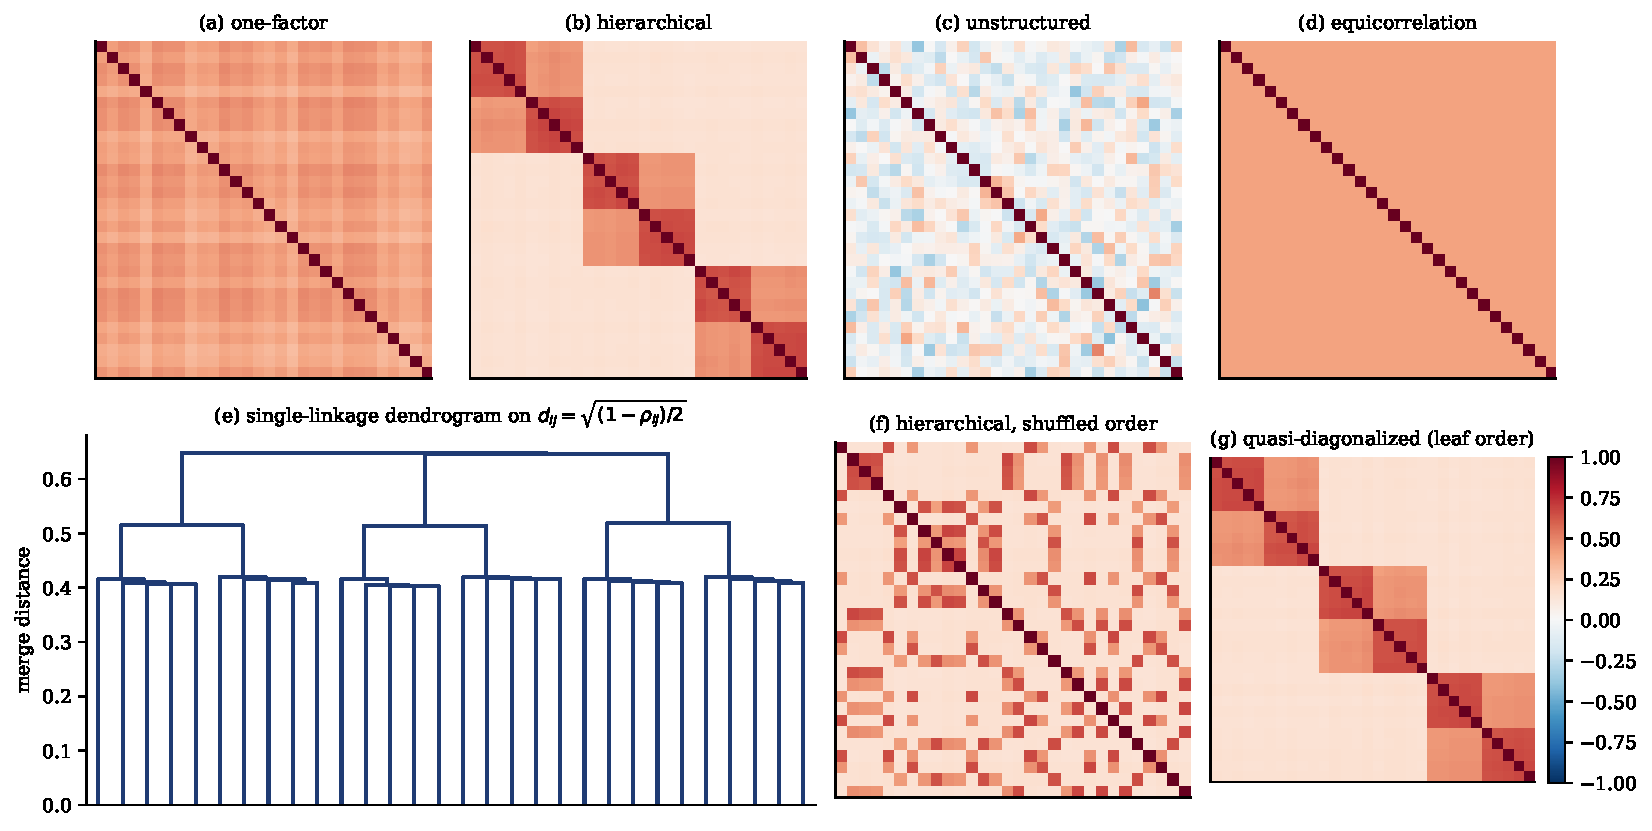
\includegraphics[width=\textwidth]{fig_setup.pdf}
\caption{The ground truth and HRP's view of it. (a--d)~True correlation
matrices from the four families (illustrative fixed configurations,
$N=30$): one-factor, nested hierarchical (three blocks, two sub-clusters
each; panel~(b) shows it in its natural block order), unstructured
normalized-Wishart, and equicorrelation.
(e)~Single-linkage dendrogram on the correlation distance
$d_{ij}=\sqrt{(1-\rho_{ij})/2}$ of the hierarchical truth. (f)~The same
hierarchical correlation matrix in the randomly permuted asset order the
allocators actually see. (g)~The matrix reordered by the dendrogram leaf
order: HRP's quasi-diagonalization recovers the block structure.}
\label{fig:setup}
\end{figure}

\section{Experimental setup}
\label{sec:setup}

We run $4{,}800$ experiments: $4{,}000$ Gaussian (seed $101$) and $800$
Student-$t$ (seed $707$), each drawing its family uniformly at random---the
Gaussian batch lands $1{,}007$ one-factor, $1{,}018$ hierarchical, $1{,}011$
unstructured, and $964$ equicorrelation experiments, with $179$--$222$
Gaussian experiments per family~$\times$~$\TN$ cell. Each experiment runs all
ten risk-track allocators and both noisy-$\mu$ directions on the same
window. All results below are stratified by family and $\TN$; we never let
an aggregate hide a family reversal, and aggregates are quoted only when the
direction agrees across families. Runs are deterministic given the released
seeds (Python 3.14.4, NumPy 2.4.6, SciPy 1.17.1, pandas 3.0.3, scikit-learn
1.9.0); the full per-experiment records ($4{,}800\times86$ fields, including
every sampled configuration value) ship with the code.

\section{Results}
\label{sec:results}

\begin{figure}[t]
\centering
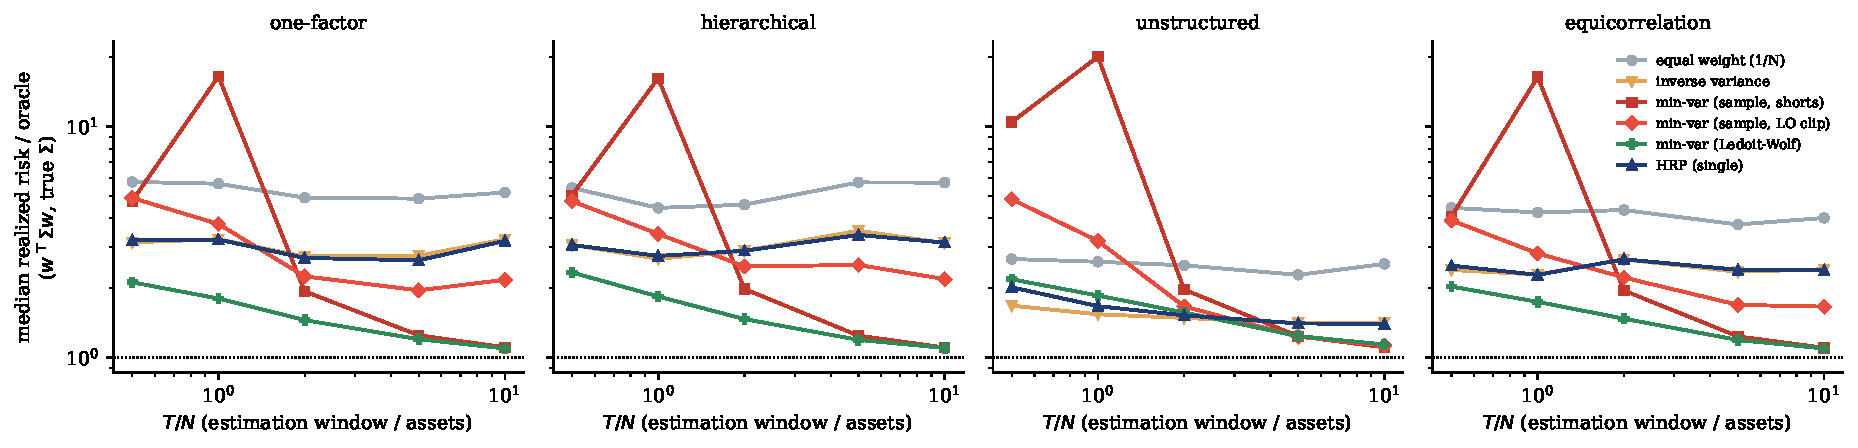
\includegraphics[width=\textwidth]{fig_risk_vs_tn.pdf}
\caption{Median realized risk relative to the oracle
(Eq.~\ref{eq:riskratio}, log--log axes) versus $\TN$, per true-structure
family ($179$--$222$ Gaussian experiments per point). Six of the ten
risk-track methods are shown; average/ward/$\tilde{d}$ HRP and LW-LO are
omitted for legibility and sit on top of their siblings
(Sections~\ref{sec:linkage} and~\ref{sec:starved}). Sample
minimum variance is catastrophic at $T\approx N$ and best-in-class by
$\TN\ge5$; Ledoit--Wolf tracks or beats HRP everywhere except the
unstructured family at $\TN\le1$; HRP and inverse variance flatten out at a
family-dependent plateau instead of converging to the oracle line at $1$.}
\label{fig:risk_vs_tn}
\end{figure}

\begin{table}[t]
\centering
\caption{Median realized risk / oracle (Eq.~\ref{eq:riskratio}) by method and
true-structure family, at the singular point $\TN=1$ and in the data-rich
regime $\TN=10$ (Gaussian batch; $180$--$212$ experiments per cell). Bold
marks each column's best method.}
\label{tab:headline}
\small
\begin{tabular}{l cccc @{\hskip 1.8em} cccc}
\toprule
& \multicolumn{4}{c}{$\TN=1$ (singular)} & \multicolumn{4}{c}{$\TN=10$ (data-rich)} \\
\cmidrule(lr){2-5}\cmidrule(lr){6-9}
Method & 1-fac. & hier. & unstr. & equi. & 1-fac. & hier. & unstr. & equi. \\
\midrule
EW ($1/N$)        & 5.65 & 4.44 & 2.60 & 4.24 & 5.18 & 5.71 & 2.54 & 4.02 \\
IV                & 3.25 & 2.68 & \textbf{1.54} & 2.29 & 3.24 & 3.13 & 1.42 & 2.41 \\
MV (sample)       & 16.45 & 16.15 & 20.00 & 16.35 & 1.11 & 1.10 & \textbf{1.11} & 1.10 \\
MV-LO (clip)      & 3.78 & 3.43 & 3.19 & 2.82 & 2.17 & 2.18 & 1.13 & 1.66 \\
LW                & \textbf{1.80} & \textbf{1.84} & 1.85 & \textbf{1.74} & \textbf{1.09} & \textbf{1.10} & 1.14 & \textbf{1.09} \\
LW-LO (clip)      & 2.88 & 2.59 & 1.85 & 2.31 & 2.20 & 2.24 & 1.15 & 1.74 \\
HRP (single)      & 3.24 & 2.75 & 1.67 & 2.28 & 3.20 & 3.14 & 1.40 & 2.38 \\
\bottomrule
\end{tabular}
\end{table}

\subsection{Data-starved regime: the insurance value is real}
\label{sec:starved}

At $\TN\le1$ the sample covariance is singular ($T-1<N$ in every such
experiment), and Eq.~\eqref{eq:minvar} on the pseudoinverse is a disaster:
pooled across families, sample MV realizes a median $16.8\times$ the oracle
risk at $\TN=1$, exceeds $10\times$ in $65\%$ of $\TN=1$ experiments and
$100\times$ in $9\%$ of them. HRP realizes a median $2.3\times$ at the same
point, equal weight $3.8\times$, inverse variance $2.2\times$
(Table~\ref{tab:headline}, left panel). HRP beats sample MV in $87\%$ of all
$\TN\le1$ experiments---in the unstructured family at $\TN=0.5$ it wins
$1.00$ of them ($201$ of $201$)---and it cannot suffer an inversion
catastrophe: its weights are positive by construction, so its worst cases are
those of any long-only rule facing an oracle that uses shorts (it exceeds
$10\times$ the oracle in $8.8\%$ of $\TN\le1$ experiments, of the same order
as EW's $19.9\%$ and IV's $8.6\%$, against $42.6\%$ for sample MV). The
practitioner folklore is, to this extent, confirmed and quantified.

Two refinements. First, the catastrophe peaks at the singularity threshold
$T\approx N$, not at the smallest sample: at $\TN=0.5$ sample MV's median is
$4.1$--$10.4\times$ by family, versus $16.2$--$20.0\times$ at $\TN=1$. With
$T\ll N$ the pseudoinverse solves the problem in a much lower-dimensional
range space, an implicit regularization; at $T\approx N$ the matrix is
invertible-but-barely, its smallest eigenvalues nearly zero, and the
optimizer amplifies them. Second, the crude long-only clip already buys back
most of the insurance: MV-LO's median at $\TN=1$ is $2.8$--$3.8\times$,
consistent with the constraints-as-shrinkage result of
\citet{jagannathan2003risk}---though it is still beaten by HRP in
$85$--$95\%$ of $\TN\le1$ experiments per family
(Table~\ref{tab:scorecard}).

\subsection{Data-rich regime: HRP does not converge}
\label{sec:rich}

The right panel of Table~\ref{tab:headline} shows the other side. By
$\TN=10$, sample MV and LW converge to ${\approx}1.10\times$ the oracle in
every family (pooled medians $1.10$ for both), and the estimation penalty is
visibly vanishing along the MV and LW curves of Figure~\ref{fig:risk_vs_tn}.
HRP's curve is flat: $3.20$ (one-factor), $3.14$ (hierarchical), $1.40$
(unstructured), $2.38$ (equicorrelation) at $\TN=10$---essentially its
$\TN=1$ values. HRP is not a consistent estimator of the minimum-variance
portfolio: more data does not help it, because its loss is dominated by a
\emph{specification} gap, not estimation error. The $\TN=10$ plateau is a
direct estimate of that gap---what HRP would lose even given the true
covariance---and it ranges from $40\%$ extra risk (unstructured) to
$220\%$ (one-factor). The same plateau afflicts inverse variance and equal
weight, which is the first hint of Section~\ref{sec:ivp}: HRP inherits its
asymptotics from the inverse-variance rule inside it. Notably, even at
$\TN=10$ the \emph{clipped} variants do not converge either (MV-LO
$1.13$--$2.18$): with an oracle that shorts, any long-only rule retains a
specification gap; what distinguishes HRP is that it carries this gap while
also being promoted as the remedy for estimation error.

\begin{table}[t]
\centering
\caption{Where HRP wins: fraction of experiments in which HRP (single
linkage) realizes strictly lower true risk than each opponent, by family,
pooled over the data-starved band ($\TN\le1$, $n=378$--$418$ per family) and
the data-rich band ($\TN\ge5$, $n=387$--$423$). Gaussian batch.}
\label{tab:scorecard}
\small
\begin{tabular}{ll cccccc}
\toprule
Band & Family & vs EW & vs IV & vs MV & vs MV-LO & vs LW & vs LW-LO \\
\midrule
$\TN\le1$ & one-factor    & 0.97 & 0.55 & 0.79 & 0.89 & 0.23 & 0.36 \\
          & hierarchical  & 0.95 & 0.41 & 0.86 & 0.90 & 0.28 & 0.37 \\
          & unstructured  & 0.76 & 0.16 & 1.00 & 0.95 & 0.55 & 0.55 \\
          & equicorr.     & 0.95 & 0.37 & 0.84 & 0.85 & 0.32 & 0.38 \\
\midrule
$\TN\ge5$ & one-factor    & 1.00 & 0.63 & 0.07 & 0.05 & 0.04 & 0.04 \\
          & hierarchical  & 1.00 & 0.60 & 0.04 & 0.03 & 0.01 & 0.02 \\
          & unstructured  & 0.95 & 0.58 & 0.08 & 0.06 & 0.06 & 0.06 \\
          & equicorr.     & 1.00 & 0.46 & 0.09 & 0.05 & 0.06 & 0.06 \\
\bottomrule
\end{tabular}
\end{table}

\begin{figure}[t]
\centering
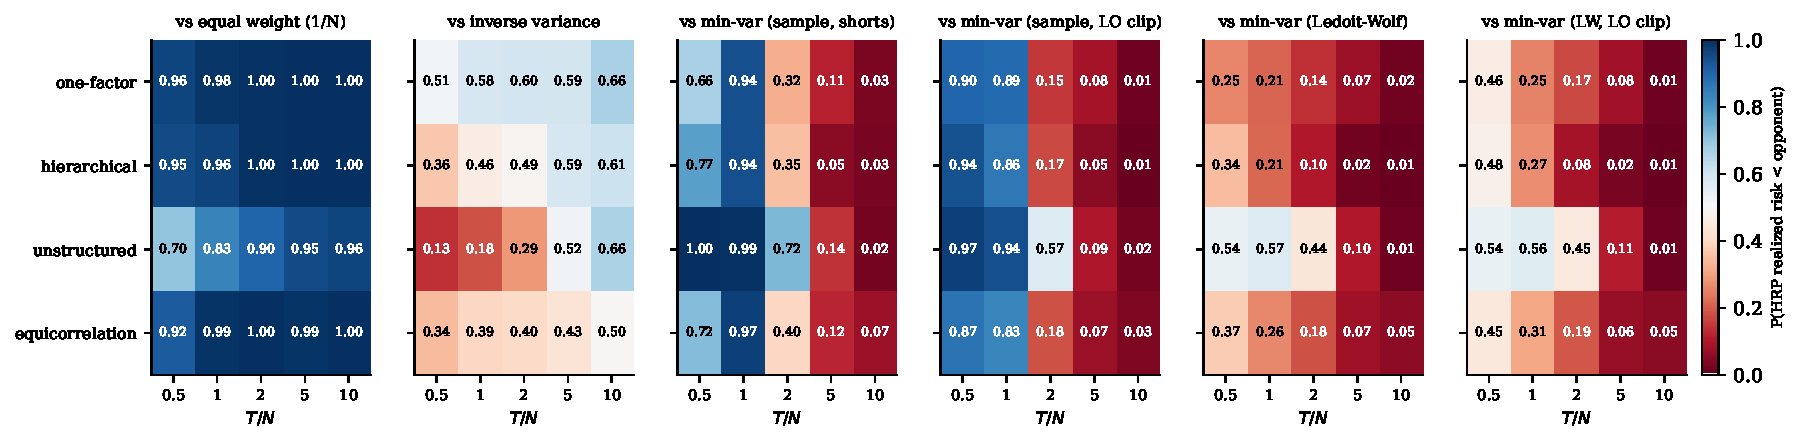
\includegraphics[width=\textwidth]{fig_winrate.pdf}
\caption{$P(\text{HRP realized risk} < \text{opponent's})$ per
family~$\times$~$\TN$ cell (Gaussian batch, $179$--$222$ experiments per
cell; blue = HRP better, red = opponent better). HRP dominates equal weight
everywhere and naive minimum variance (with or without the long-only clip)
wherever $\TN\le1$; against Ledoit--Wolf it is below $0.5$ in every cell of
the one-factor, hierarchical, and equicorrelation families, with the
unstructured small-$T$ corner (win rates $0.54$--$0.57$) the lone
exception. Against inverse variance HRP hovers near $0.5$ except in the
unstructured family at small $T$, where the clustering machinery actively
hurts ($0.13$--$0.29$).}
\label{fig:winrate}
\end{figure}

\subsection{The honest headline: shrinkage beats HRP almost everywhere}
\label{sec:shrinkage}

Table~\ref{tab:headline} already shows it in medians; Table~\ref{tab:scorecard}
and Figure~\ref{fig:winrate} show it experiment by experiment. Ledoit--Wolf
minimum variance---which fixes the same singularity HRP fixes, with one line
of scikit-learn---realizes lower true risk than HRP at \emph{every} $\TN$ in
the one-factor, hierarchical, and equicorrelation families. Pooled across
families, HRP's win rate against LW is $0.34$ at $\TN\le1$ and falls to
$0.05$ at $\TN\ge5$. The single exception is the unstructured family at
small $T$: with nothing for the shrinkage target (or the dendrogram) to
exploit, HRP edges LW with win rates of $0.54$ at $\TN=0.5$ and $0.57$ at
$\TN=1$, and a median paired log-ratio near zero ($-0.02$ dex at
$\TN=1$).\footnote{Even this corner is not uniform: stratified by universe
size, HRP's win rate against LW in the unstructured $\TN\le1$ pool is
$0.34$ at $N=10$, $0.59$ at $N=30$, $0.60$ at $N=50$, and $0.69$ at
$N=100$. At $N=10$ LW is ahead even here; the exception is a large-$N$,
small-$T$ phenomenon.}
Even this
exception deflates on inspection: in the same cells, plain inverse variance
is better still (median $1.54\times$ vs.\ HRP's $1.67\times$ at $\TN=1$; HRP
beats IV in only $0.16$ of unstructured $\TN\le1$ experiments). Where HRP
beats shrinkage, it does so not because clustering helps but because
\emph{correlations are pure noise there and HRP mostly ignores them}---and
the allocator that ignores them entirely wins.

It is worth being precise about what HRP wins against, because the
practitioner comparison is usually HRP versus naive Markowitz: against
sample MV and the clipped MV-LO at $\TN\le1$, HRP wins $0.79$--$1.00$ of
experiments per family. The insurance is real; it is the choice of
comparator that flatters HRP. Against the equally inversion-proof
LW, the picture inverts almost everywhere.

\subsection{HRP is mostly the inverse-variance portfolio inside it}
\label{sec:ivp}

Against diagonal inverse variance, HRP's win rates hover near $0.5$ in most
cells (Table~\ref{tab:scorecard}, ``vs IV''), and the median paired
log-ratios are tiny (within $\pm0.006$ dex, i.e.\ $\pm1.5\%$ in risk, in
every hierarchical-family cell). The pattern splits by band: with ample data
HRP is modestly ahead of IV in three of four families (win rates
$0.46$--$0.63$ at $\TN\ge5$), while in the data-starved band the clustering
machinery earns its keep only where the truth has the specific asymmetry it
is built to exploit. Our
hierarchical generator makes that asymmetry an explicit, sampled parameter:
\texttt{block\_disp} scales each cluster's variance share by
$U(1-d,1+d)$, so $d=0$ gives equally tight clusters (inverse variance
near-optimal by symmetry) and large $d$ gives clusters of very different
tightness. Within the hierarchical family at $\TN\le2$, HRP's win rate
against IV rises monotonically across \texttt{block\_disp} terciles: $0.35$
(mean $d=0.13$), $0.40$ (mean $d=0.38$), $0.56$ (mean $d=0.66$). The median
paired advantage remains small even in the top tercile ($-0.002$ dex,
${\approx}0.4\%$ less risk), so the dispersion effect is real but modest in
magnitude---and note that against LW the same terciles read
$0.28/0.19/0.19$: cluster asymmetry helps HRP relative to its own diagonal
core, not relative to shrinkage. In short: most of HRP's behavior is the
IVP; the dendrogram adds a structure-conditional refinement, not a
transformation.

\subsection{Linkage does not matter (and turnover diagnostics)}
\label{sec:linkage}

Practitioner debate spends considerable energy on the linkage rule, citing
single linkage's chaining pathology \citep{murtagh2012algorithms} and
preferring average or Ward variants \citep{raffinot2017hierarchical}. On the
minimum-variance criterion the choice is immaterial in our testbed: the
median realized-risk ratios of single/average/ward HRP per family agree to
$2.95/2.93/3.00$ (one-factor), $3.04/3.06/3.04$ (hierarchical),
$1.57/1.53/1.54$ (unstructured), and $2.42/2.42/2.39$
(equicorrelation)---the three linkage medians agree to within
$0.02$--$0.06$ (Figure~\ref{fig:sensitivity}a), a disagreement one to two
orders of magnitude smaller than the gaps between allocator families in
Table~\ref{tab:headline}. No linkage is best in more than two families, and
which one ``wins'' flips across families. Anyone tuning HRP should tune
\emph{whether} to cluster, not \emph{how} to link.

The distance-matrix convention matters just as little, which doubles as a
faithfulness check on our implementation (Section~\ref{sec:allocators}):
recomputing single-linkage HRP with the linkage on the Euclidean
distance-of-distances $\tilde{d}$---the matrix the original code listing
hands to the clustering routine---moves the per-family median risk ratio by
at most $0.02$ ($2.95\to2.94$ one-factor, $3.04\to3.05$ hierarchical,
$1.57\to1.58$ unstructured, $2.42\to2.44$ equicorrelation), with a paired
median log-ratio of exactly zero and a $\tilde{d}$ win rate of
$0.44$--$0.48$ per family. The per-experiment weights genuinely differ---the
two conventions realize bit-identical risk in only $4$--$9\%$ of
experiments---but no aggregate conclusion in this paper changes under either
convention.

The same figure reports two operational diagnostics. Concentration
(Figure~\ref{fig:sensitivity}b): all methods are diffuse in median terms
(gross-weight Herfindahl $0.02$--$0.08$), with HRP (${\approx}0.04$) close
to IV and LW; the optimizers are not visibly more concentrated in the
median---their pathology is instability, not static concentration, and
sample MV holds a median gross short position of $0.57$ versus $0.25$ for
LW. Estimation-noise turnover (Figure~\ref{fig:sensitivity}c) makes the
instability explicit: redrawing the estimation window from the same truth
moves sample MV's weights by a median half-$L_1$ distance of $4.43$ at
$\TN=1$---more than four times the entire book---versus $0.52$ for LW,
$0.22$ for HRP, and $0.12$ for IV. HRP's practical appeal of low, stable
turnover is genuine; it is inherited from the near-diagonal allocation, and
LW pays roughly twice HRP's turnover for its risk advantage.

\begin{figure}[t]
\centering
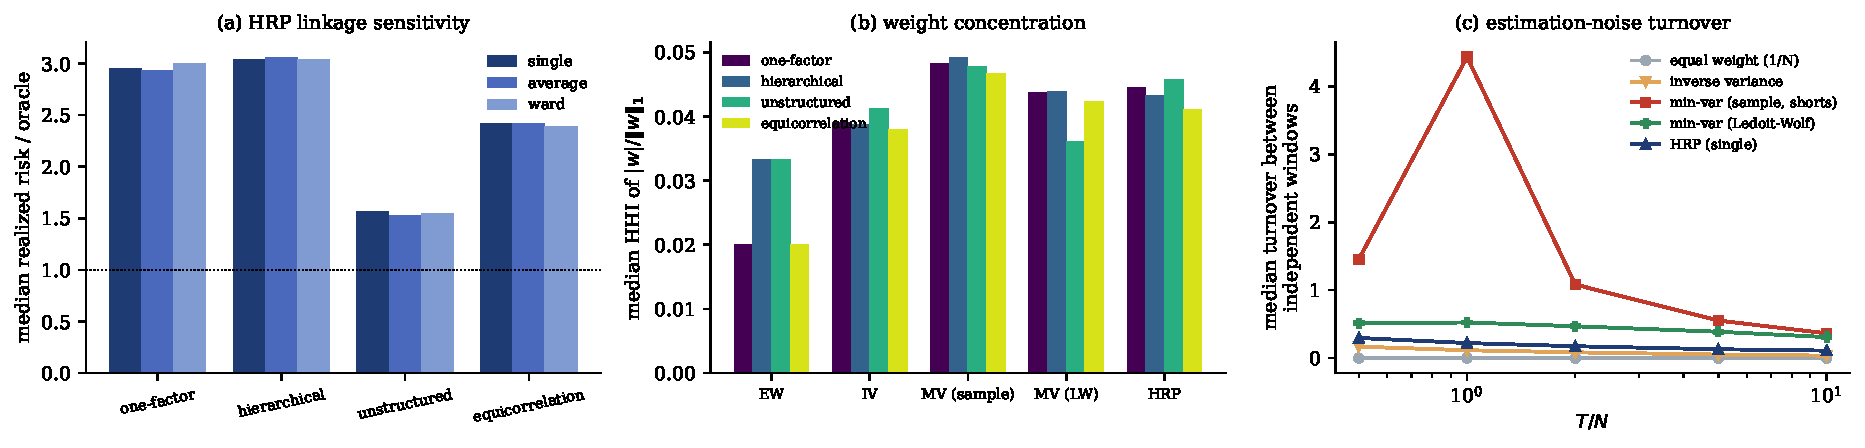
\includegraphics[width=\textwidth]{fig_sensitivity.pdf}
\caption{(a)~Linkage sensitivity: median realized risk / oracle for
single/average/ward HRP, by family (all $\TN$ pooled); the spread within
each family is $0.02$--$0.06$. (b)~Median concentration (Herfindahl index of
$|w|/\lVert w\rVert_1$) by method and family: every method is diffuse in the
median; EW's $1/N$ differs across families only through their $N$ mixes.
(c)~Estimation-noise turnover: median $\tfrac12\lVert
w^{(1)}-w^{(2)}\rVert_1$ between two independent windows drawn from the same
truth, by $\TN$ (all families pooled). Sample minimum variance peaks at
$4.43$ at the singularity threshold $\TN=1$; HRP stays at $0.11$--$0.30$,
below Ledoit--Wolf throughout.}
\label{fig:sensitivity}
\end{figure}

\subsection{Estimated means are the real catastrophe}
\label{sec:mu}

Everything above concerns risk-only allocators, which is where the
HRP-versus-shrinkage debate lives. For perspective, the same harness runs
the classical Markowitz tangency direction with \emph{estimated} means,
$\Sighat^{+}\muhat$, and scores its true Sharpe ratio against the oracle
tangency ceiling $\sqrt{\mu^{\top}\Sig^{-1}\mu}$
(Table~\ref{tab:sharpe}). At $\TN\le1$ the noisy-$\mu$ direction captures a
median $8$--$11\%$ of the attainable Sharpe ratio by family (pooled
$10\%$), and its true Sharpe ratio is \emph{negative}---the estimated
direction points the wrong way---in $28\%$ of experiments. Shrinking the
covariance inside the tangency formula helps ($19$--$22\%$ captured) but
does not rescue it; the failure is in $\muhat$, reproducing
\citet{demiguel2009optimal} and the error-sensitivity hierarchy of
\citet{chopra1993effect} inside a fully controlled environment. By contrast,
the three $\mu$-free rules of Table~\ref{tab:sharpe} capture $26$--$70\%$ in
the same regime, and even the weakest $\mu$-free allocator on this track,
sample minimum variance, captures a pooled median $18\%$ (per-family medians
$0.15$--$0.25$)---nearly twice the noisy-$\mu$ direction. Even with
ten observations per asset, noisy-$\mu$ tangency captures only $48$--$71\%$
and is still negative in $2$--$6\%$ of experiments.

Two honest caveats from the same table. First, minimum variance is not the
Sharpe-optimal objective: the \emph{oracle} minimum-variance portfolio
itself captures only $0.20$--$0.26$ of the tangency Sharpe in the three
structured families (it captures $0.84$--$0.85$ in the unstructured family,
where the tangency and minimum-variance portfolios nearly coincide under our
mean model). Equal weight and HRP, whose Sharpe capture ($0.34$--$0.44$ in
structured families) \emph{exceeds} the oracle minimum-variance floor's,
profit from a mean model in which all assets have similar expected Sharpe
ratios---a regime that flatters diffuse portfolios on the Sharpe track,
exactly as the $1/N$ literature would predict. Second, these Sharpe-track
numbers therefore do not contradict the risk-track ranking; they answer a
different question (``how much Sharpe, given this mean structure?'' versus
``how close to the minimum-variance floor?'').

\begin{table}[t]
\centering
\caption{Sharpe track: median true Sharpe ratio as a fraction of the oracle
tangency ceiling, by family and $\TN$ band (Gaussian batch). MV-$\mu$ and
MV-$\mu$-LW are tangency directions built from estimated means with the
sample and Ledoit--Wolf covariance; ``neg.'' is the fraction of experiments
with negative true Sharpe ratio for MV-$\mu$; the last column is the
\emph{oracle} minimum-variance portfolio's own capture (the ceiling for the
risk-only rules under this mean model).}
\label{tab:sharpe}
\small
\begin{tabular}{ll ccc cc c c}
\toprule
Band & Family & EW & LW & HRP & MV-$\mu$ & MV-$\mu$-LW & neg. & or.\ MV \\
\midrule
$\TN\le1$ & one-factor    & 0.37 & 0.26 & 0.36 & 0.11 & 0.22 & 0.28 & 0.20 \\
          & hierarchical  & 0.40 & 0.30 & 0.39 & 0.10 & 0.21 & 0.29 & 0.22 \\
          & unstructured  & 0.66 & 0.70 & 0.57 & 0.11 & 0.20 & 0.23 & 0.84 \\
          & equicorr.     & 0.40 & 0.28 & 0.39 & 0.08 & 0.19 & 0.33 & 0.23 \\
\midrule
$\TN\ge5$ & one-factor    & 0.34 & 0.23 & 0.36 & 0.55 & 0.56 & 0.05 & 0.24 \\
          & hierarchical  & 0.36 & 0.21 & 0.36 & 0.56 & 0.57 & 0.06 & 0.21 \\
          & unstructured  & 0.67 & 0.82 & 0.67 & 0.71 & 0.64 & 0.02 & 0.85 \\
          & equicorr.     & 0.44 & 0.26 & 0.44 & 0.48 & 0.50 & 0.06 & 0.26 \\
\bottomrule
\end{tabular}
\end{table}

\subsection{Student-$t$ robustness}
\label{sec:studentt}

The $800$-experiment multivariate Student-$t$ batch ($\nu\sim U(4,10)$,
covariance rescaled to exactly $\Sig$) reproduces every qualitative ranking
(Table~\ref{tab:studentt}). Fat joint tails make the inversion-based
estimators a little worse in every family (sample MV by $+0.04$ to $+0.25$
in the median, LW by $+0.02$ to $+0.11$); the diffuse rules move by up to
$1.1$ in the noisier $193$--$205$-experiment $t$-cells without changing
sign or order anywhere. HRP's win rate against LW by family is
$0.13$--$0.38$ under Student-$t$ versus $0.14$--$0.32$ under Gaussian
sampling, with the unstructured family again the most HRP-friendly and the
one-factor family the least. Fatter tails do not reorder the comparison.

\begin{table}[t]
\centering
\caption{Gaussian vs.\ Student-$t$ sampling: median realized risk / oracle
by family (all $\TN$ pooled; $964$--$1{,}018$ Gaussian and $193$--$205$
Student-$t$ experiments per family), and HRP's win rate against Ledoit--Wolf
in the same pool.}
\label{tab:studentt}
\small
\begin{tabular}{ll cccc c}
\toprule
Returns & Family & EW & MV & LW & HRP & win HRP vs LW \\
\midrule
Gaussian    & one-factor    & 5.24 & 1.90 & 1.41 & 2.95 & 0.14 \\
            & hierarchical  & 5.22 & 1.97 & 1.43 & 3.04 & 0.14 \\
            & unstructured  & 2.51 & 1.88 & 1.48 & 1.57 & 0.32 \\
            & equicorr.     & 4.14 & 1.82 & 1.34 & 2.42 & 0.19 \\
\midrule
Student-$t$ & one-factor    & 5.14 & 2.05 & 1.48 & 3.19 & 0.13 \\
            & hierarchical  & 4.16 & 2.22 & 1.47 & 2.50 & 0.18 \\
            & unstructured  & 2.48 & 2.08 & 1.60 & 1.73 & 0.38 \\
            & equicorr.     & 4.47 & 1.86 & 1.36 & 2.65 & 0.19 \\
\bottomrule
\end{tabular}
\end{table}

\section{Discussion}
\label{sec:discussion}

\paragraph{When should one actually use HRP?} Our results support a narrow
but real use case: \emph{covariance structure unknown or plausibly
unstructured, and $T\lesssim N$}. There HRP matches Ledoit--Wolf (win
${\approx}0.55$), never explodes, and turns over a twentieth as much as
unconstrained sample MV ($0.22$ vs.\ $4.43$ at $\TN=1$) and a third as much
as the clipped variant. If one believes the truth is dense random correlation, plain
inverse variance is better still; HRP is the hedge for not knowing. In every
structured world we tested---one common factor, genuine nested hierarchy
(the case HRP was designed for!), constant correlation---Ledoit--Wolf
shrinkage realized less true risk at every $\TN$, with win rates against
HRP of $0.63$--$0.99$ per cell. The deepest irony of the comparison is that
HRP loses most clearly in the hierarchical family itself: knowing that the
truth is hierarchical is covariance information, and the estimator that uses
all of $\Sighat$ (gently shrunk) exploits it better than a greedy dendrogram
that uses only the ordering it induces.

\paragraph{What the plateau means.} Because the oracle is exact, the
$\TN\to10$ limit cleanly separates the two failure modes that backtests
confound. The optimizers' excess risk is almost entirely estimation error
(it vanishes: $1.10\times$ at $\TN=10$); HRP's is almost entirely
specification error (it persists: $1.40$--$3.20\times$). The practical
corollary: more history helps Markowitz-type rules and does essentially
nothing for HRP, so the break-even $\TN$ between them is not a constant of
nature but falls out of the data: HRP's win rate against sample MV crosses
$0.5$ between $\TN=1$ and $2$ in the three structured families and between
$2$ and $5$ under unstructured correlation. This locates HRP
and minimum variance at the two ends of the Schur-complement continuum of
\citet{cotton2024schur} along an \emph{estimation-error} axis: our results
say to sit near the HRP end only briefly, and to slide toward the
(shrunk) MV end as soon as $T$ permits.

\paragraph{What HRP's machinery actually contributes.} The decomposition
across Sections~\ref{sec:ivp}--\ref{sec:linkage} is unflattering to the
celebrated parts of the algorithm. The dendrogram's linkage rule is
irrelevant (median spreads of $0.02$--$0.06$, and at most $0.02$ for the
distance-matrix convention); the quasi-diagonalization matters only
through the bisection it enables; and in the data-starved band the bisection
improves on diagonal inverse variance only when clusters differ materially
in tightness (\texttt{block\_disp} terciles: $0.35\to0.56$ win rate vs IV),
by a median margin under half a percent of risk---with ample data it edges
IV more broadly (win rates $0.46$--$0.63$ at $\TN\ge5$), but those wins do
not close the gap to shrinkage. HRP's robustness---the property that
sells it---comes from the part nobody advertises: it is approximately an
inverse-variance portfolio, and inverse variance is hard to break. Stated
plainly: if you want HRP's safety, IV gives you most of it; if you want
optimality, shrinkage gives you more of it; HRP's niche is the intersection
where you want a long-only, inversion-free rule that still reacts a little
to cluster structure.

\paragraph{Means remain the priority.} Nothing in the covariance debate
compares to the damage of estimating means: a median $90\%$ of attainable
Sharpe destroyed at $\TN\le1$, with the direction outright wrong in $28\%$
of experiments. Practitioners arguing HRP versus shrinkage while feeding
estimated means into anything have, in our measurements, chosen the wrong
battle by an order of magnitude.

\section{Limitations}
\label{sec:limitations}

Returns in our testbed are i.i.d.\ across time---Gaussian in the main batch,
multivariate Student-$t$ (common mixing variable, $\nu\in[4,10]$) in the
robustness batch---and the true covariance is constant over the estimation
window. Real returns exhibit autocorrelation, volatility clustering, regime
switches, and asymmetric tail dependence; all of these degrade every
estimator, and dynamics that mimic block structure intermittently could
shift the HRP-versus-shrinkage margin in either direction. Our evaluation is
single-period with no transaction costs: we report estimation-noise turnover
as a diagnostic but do not net it against risk performance, which would
favor HRP and IV. The long-only variants use the crude clip-and-renormalize
heuristic rather than the constrained quadratic program, deliberately (it is
what naive implementations do), so our MV-LO and LW-LO numbers are lower
bounds on what proper constrained optimization achieves. We likewise test a
single shrinkage estimator---Ledoit--Wolf toward a scaled identity; the
constant-correlation target \citep{ledoit2004honey}, the factor target
\citep{ledoit2003improved}, and nonlinear shrinkage are untested, and the
lone unstructured small-$T$ corner where HRP edges LW might not survive a
better-matched target. The oracle floor
allows short positions, so long-only rules carry a structural specification
gap in the risk ratio; this affects levels, not the paired comparisons
between long-only methods. Our four families, though spanning factor,
hierarchical, dense-random, and equicorrelated worlds, are all static linear
structures---three with positive mean correlation, while the unstructured
family's mean off-diagonal correlation is approximately zero---and the mean
model
($\mu_i=s_i\sigma_i$ with similar per-asset Sharpe ratios) is one
defensible choice among several; the Sharpe-track levels in
Table~\ref{tab:sharpe} depend on it, though the risk-track results do not
use means at all. Finally, we test HRP as specified in the original paper
plus linkage variants; extensions (HERC, constrained or Schur-blended
versions) may behave differently and can be dropped into the released
harness.

\section{Conclusion}
\label{sec:conclusion}

We measured Hierarchical Risk Parity against Markowitz-type and shrinkage
allocators in a controlled environment where the true covariance is known
and every realized risk is exact. The popular story is half right. HRP's
insurance value against naive sample minimum variance is real and large: at
$T=N$ the optimizer realizes a median $16.8\times$ the attainable risk
floor and HRP $2.3\times$, winning $87\%$ of data-starved comparisons. But
against Ledoit--Wolf shrinkage---which cures the same singularity at the
same computational cost---HRP loses at every $\TN$ in every structured
family we tested, including the nested-hierarchical worlds it was designed
for, winning only in the unstructured small-$T$ corner where its own
diagonal core (inverse variance) is better still. HRP does not converge to
the optimum as data grows (plateau at $1.40$--$3.20\times$), its
much-debated linkage choice moves family medians by $0.02$--$0.06$, and its
genuine advantages---no inversion, positive weights, low estimation-noise
turnover---are inherited from the inverse-variance portfolio it wraps.
Estimated means remain the catastrophe that dwarfs the covariance debate:
noisy-$\mu$ tangency captures a median $10\%$ of attainable Sharpe at
$\TN\le1$ and points the wrong way $28\%$ of the time. Use HRP when the
structure is unknown and the window is short; shrink when you can; and
treat any allocator that needs estimated means as the actual emergency.

\paragraph{Reproducibility.} All experiments are deterministic given the
released seeds ($101$ Gaussian, $707$ Student-$t$); the script
\texttt{scripts/run\_all.py} regenerates every record, summary, and figure
input (\texttt{results/results.json}, \texttt{results/records.csv}, $4{,}800$
experiments $\times$ $86$ recorded fields), \texttt{python -m
hrp\_experiments.figures} regenerates the four figures, and
\texttt{scripts/check\_paper\_numbers.py} verifies that every number quoted
in this paper matches the generated results. The covariance generator
(Table~\ref{tab:ranges} is its complete parameter space), allocators,
simulation harness, and analysis are provided as an open-source package at
\url{https://github.com/suenot/hrp-validation}.

\small
\bibliographystyle{plainnat}
\bibliography{refs}

\end{document}
